% !TEX TS-program = xelatex
% !TEX encoding = UTF-8

\documentclass[a4paper,11pt]{article} % use larger type; default would be 10pt
\usepackage{../skills-analysis/default}
\usepackage{graphicx}

\ifxetex
\setmainfont{Droid Sans}
\setmonofont[Scale=0.9]{Droid Sans Mono}
\linespread{1.3}
\fi

\usepgfplotslibrary{fillbetween}

\title{Project Report --- Lumberjack}
\author{Joe MacMahon}
\date{\today}

\begin{document}
\maketitle

\section{Introduction}
\label{sec:introduction}
% TODO dot dot dot
As a part of my placement at CERN, I developed a software library called
Lumberjack over the course of several months.  This will be a critical
evaluation of that project, including some context of why I developed it, an
in-depth view of two interesting areas in its development, and also some
surrounding information about my placement itself.

\subsection{CERN Profile}
\label{sec:cern}
CERN, the European Organisation for Nuclear Research is a world-famous research
facility for particle physics located on the French-Swiss border, just outside
Geneva.  It was founded in 1954 (recently celebrating its 60th anniversary) and
currently has 21 member states from which it receives funding, and since that
time has been responsible for some of the world's most important achievements
in particle physics.

Such a large scientific operation obviously requires a substantial computing
infrastructure to support it, and as such CERN has made significant
contributions to the world of computing.  It is famous as the place where Tim
Berners-Lee created the first incarnation of the World Wide Web in 1991, and
more recently it has been known for developments in grid computing with the LHC
Computing Grid.

In terms of management structure, CERN is composed of a three-layer heirarchy:
there are eight departments\footnote{Beams; Engineering; Finance, Procurement
  and Knowledge Transfer; General Infrastructure Services; Human Resources;
  Information Technology; Physics and Technology}, each of which is divided
into a number of groups, and the groups are divided into sections.  My section,
for example, is IT-CIS-DLS, which means the IT department, Collaboration \&
Information Services (CIS) group, Digital Library Servces (DLS) section.
Ultimately the head of the organisation is the CERN council, which is made up
of delegates from each member state, and the day-to-day top-tier management is
undertaken by the Director-General, appointed for five years by the council.

% TODO talk about tech students

After a shutdown period of more than a year, CERN has just started the second
run of its principle particle accelerator, the Large Hadron Collider, colliding
particles at energies higher than ever previously observed.  This will mean
lots of publication and productive research activity over the coming months and
years and will continue to set the pace of global particle physics research.

\section{Context}
\label{sec:context}
My technical student project at centres on the CERN Document Server, which is a
service to manage papers, reports, press releases, bulletins and multimedia
created at CERN.  It also manages the library's loan system and journal
subscriptions, and provides access to peer-reviewed articles in high-energy
physics to CERN members.  The software that runs CDS is called Invenio, and
also powers a family of other sites as well, for example Inspire and Zenodo.

As with many other large services, a system for gathering and visualising usage
data is important.  In Invenio version 1 this is achieved by logging data to
MySQL and then generating graphs serverside viewable by an administrator;
however, this approach doesn't scale well when a service grows to the size of
CDS.  So, my project is to implement a new system for usage data and analytics
based on Elasticsearch, which is a distributed data store and search engine.

The scope of this report concerns the logging aspect, although my overarching
project also includes implementing visualisations of the logged data.

Since Invenio is written in Python, we decided on using the standard Python
logging system to collect our event data.  It's easy to use since it avoids
lots of object-passing through the main application; it's standard and
therefore stable and well-tested; plus its heirarchical logging system enables
us to keep logs going to Elasticsearch within their own namespace, to make sure
ordinary debug or warning logs stay out of the Elasticsearch ecosystem.

\subsection{Outline of Python Logging}
\label{sec:pythonlogging}
The Python logging system operates on a system of named \snip{Logger}
objects, accessible by the \snip{logging.getLogger()} function.  To access a
\snip{Logger} named \snip{web}, for example, you would call
\snip{logging.getLogger('web')}.  Once you have a \snip{Logger} object, you
can log an event or message by calling its \snip{.log()} method, with an
optional severity level, and for convenience, methods called \snip{.debug()},
\snip{.info()}, and \snip{.warn()}, \snip{.error()} are also provided,
with an implicit severity level for each.

Any \snip{Logger} object can have a \snip{LogHandler} object added to it,
to which log events are passed if they are of a high enough severity level.
The handler can, for example, write to a file, write to standard error, or
simply discard all events passed to it, depending on the implementation, and a
number of handlers are provided out-of-the-box with the logging library.

The loggers are arranged in a tree structure, with names separated by dots.
For example a logger named \snip{web.pageviews} is a child of \snip{web},
which itself is a child of the singleton `root' logger.  By default, if there
are no handlers attached to a logger when an event is logged, then it is passed
up the tree to the parent logger where the process begins again.

This design allows for complex and powerful logging structures, that can be
used to direct log data from different parts of an application to different
places, or turn debug-level logging on from one aspect while keeping only
error-level messages from another.

However, there is no built-in \snip{LogHandler} to send log events to
Elasticsearch, and (more surprisingly) there were no third-party libraries to
provide one either.

\autoref{fig:pythonlogging.flowdiagram} contains a schematic diagram of how
logs are processed.

\begin{figure}[h]\centering
  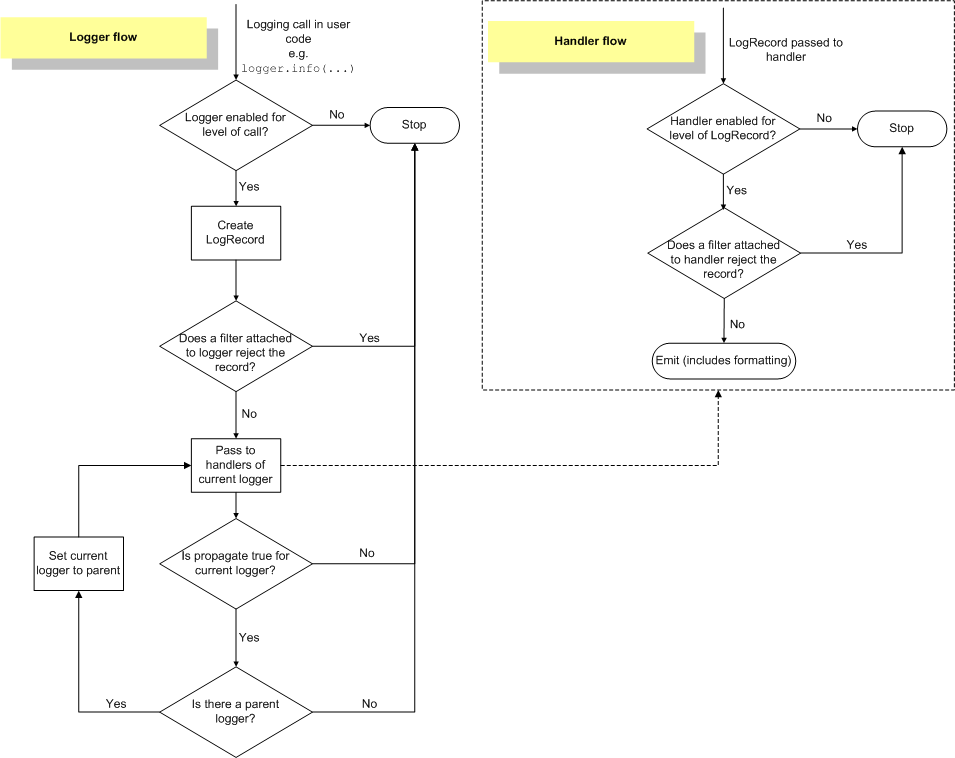
\includegraphics[width=\textwidth]{logging_flow}
  \caption{The flow of log event information.\protect\footnotemark}
\label{fig:pythonlogging.flowdiagram}
\end{figure}
\footnotetext{Copyright Python Software Foundation; PSFL licence.  Source: \url{https://docs.python.org/2/howto/logging.html}}

\section{Proposal}
\label{sec:proposal}
Faced with this issue, we decided it would be a good idea to develop our own
library to connect the two systems.  It would provide a handler to attach to a
logger in the heirarchy, and forward events expressed as Python \snip{dict}
objects to Elasticsearch over the REST API.  It should also be tolerant to use
cases other than our own by accepting standard string-based log messages.

\section{Implementation}
\label{sec:implementation}
In this section, we will give an overview of how the library works, and then
move on to an in-depth look at two aspects of its development.

\subsection{Outline of Lumberjack}
\label{sec:implementation.lumberjack}
The crux of the library is to provide a \snip{LogHandler} object which will
send events that it receives on to Elasticsearch.  This is attached to a
\snip{Logger} object on application setup, and then events are passed to this
\snip{Logger} in the standard way.  Lumberjack needs to know what
Elasticsearch index to send data to, so we use a factory pattern to generate
parametrised \snip{LogHandler} objects.  We then attach these to the
\snip{Logger} at the root of our particular namespace.

In Python pseudo-code:
\begin{lstlisting}[language=Python,basicstyle=\ttfamily]
import logging
import lumberjack
lj = lumberjack.Lumberjack( ... some global initialisation parameters ... )

myHandler = lj.getHandler(index='my-elasticsearch-index')
myLogger = logging.getLogger('some_namespace')
myLogger.addHandler(myHandler)
\end{lstlisting}

\autoref{fig:implementation.initialisation_step} contains a diagram
representation of this process.

\begin{figure}[h]
  \centering
  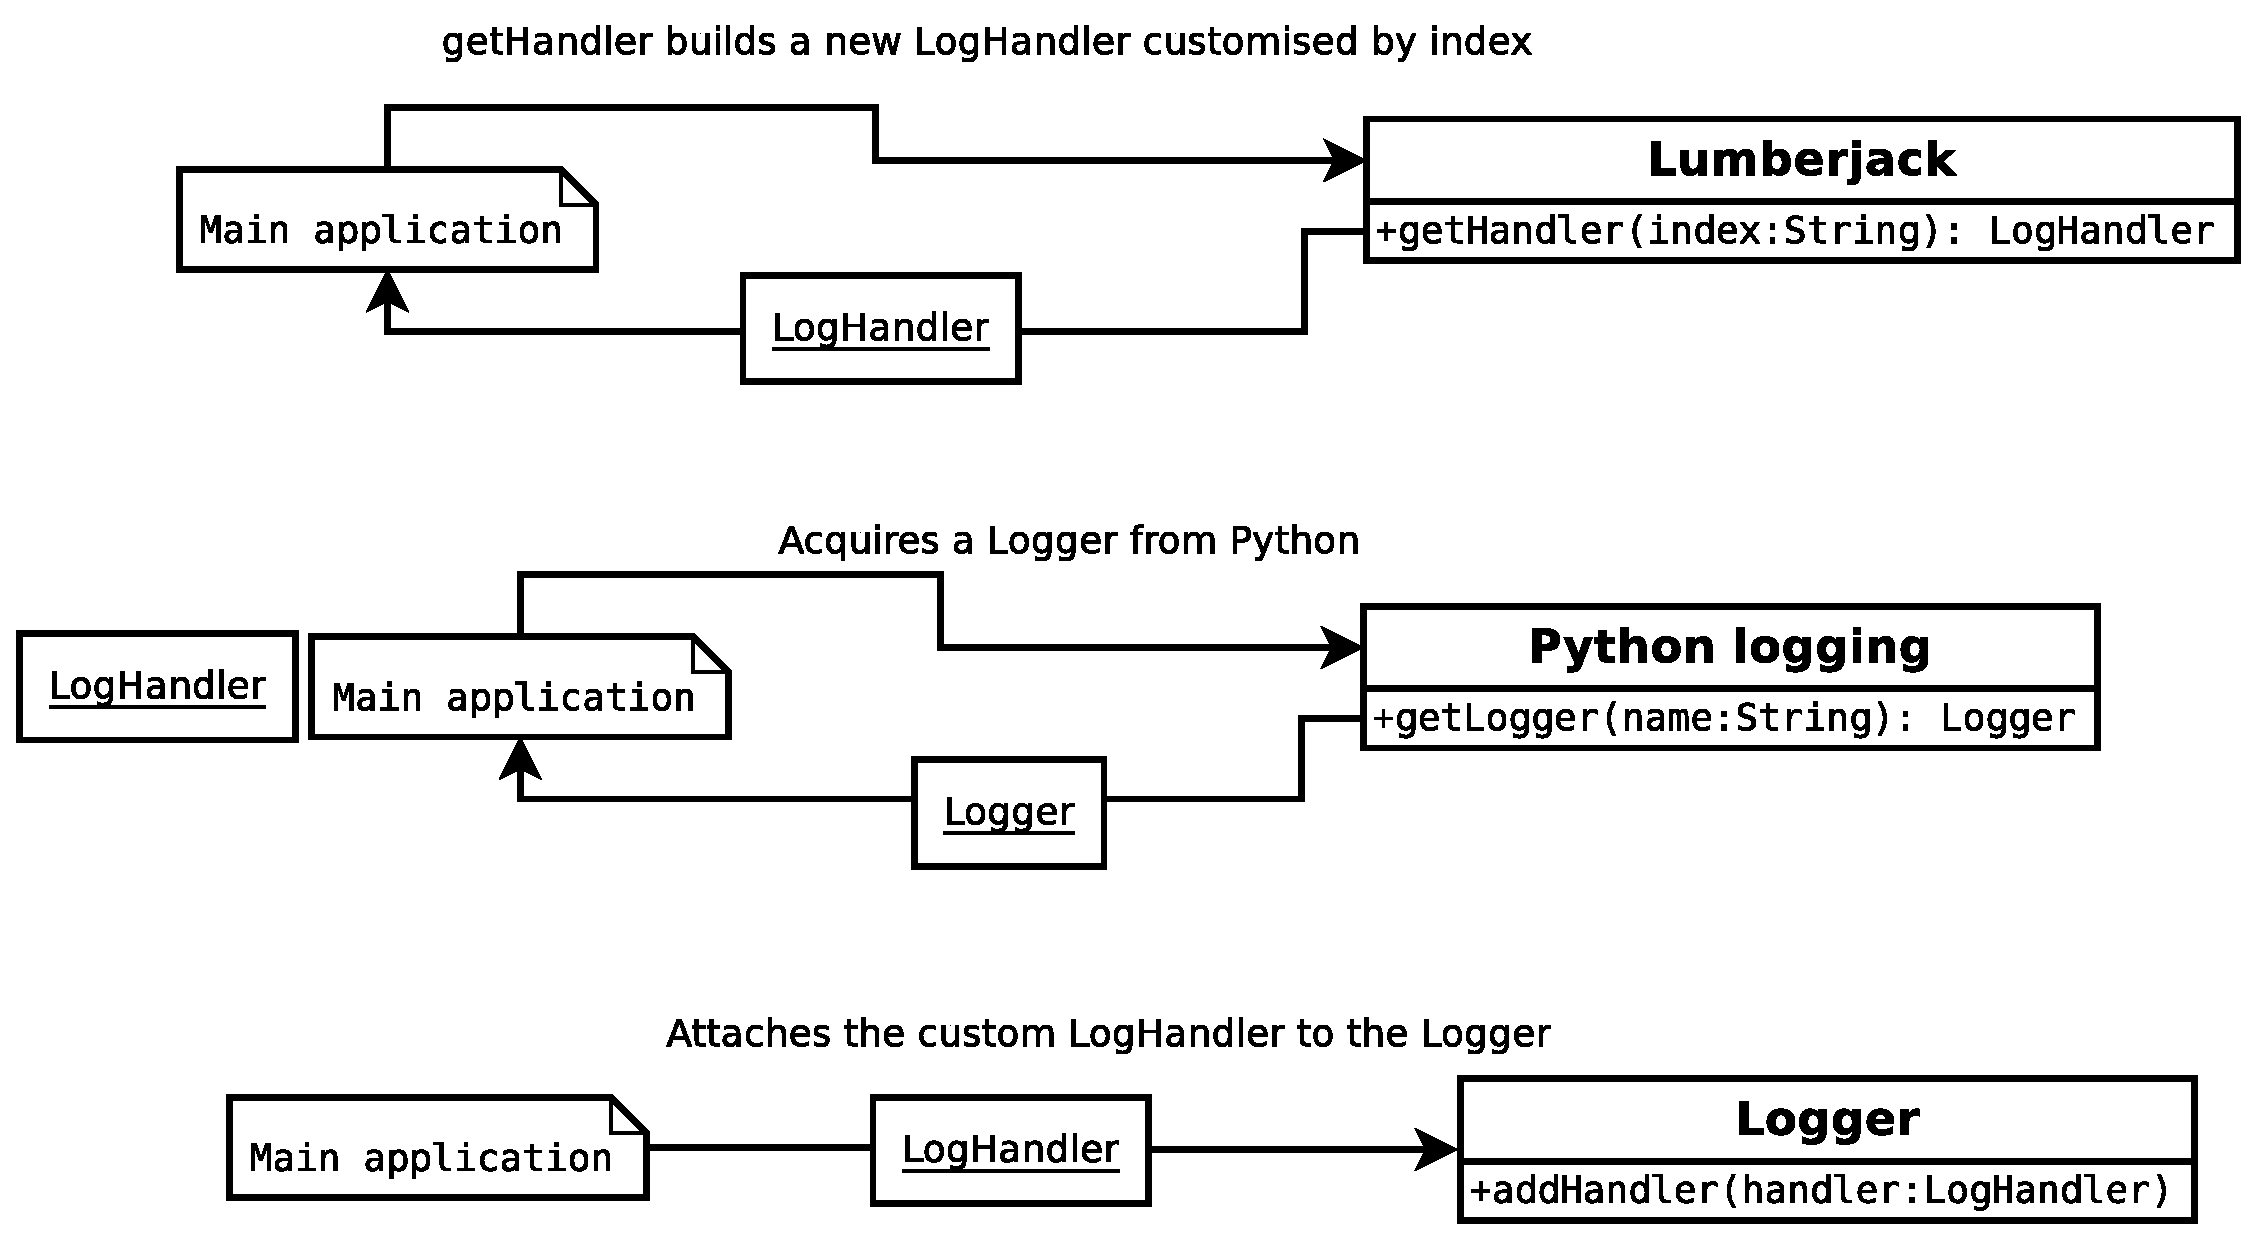
\includegraphics[width=\textwidth]{initialisation_step}
  \caption{Initial process for attaching a Lumberjack handler to a Python Logger}
  \label{fig:implementation.initialisation_step}
\end{figure}

Once initialisation is finished, the main application should then use the
standard \snip{Logger} methods, \snip{.info()}, \snip{.warn()}, etc., to
pass an event into Elasticsearch.  The custom log handler adds some metadata
(timestamp, severity level, logger name), and sends the augmented event data to
Elasticsearch.  To do this it uses the official Python Elasticsearch interface
library.

Again in Python pseudo-code:

\begin{lstlisting}[language=Python,basicstyle=\ttfamily]
import logging

event_A_logger = logging.getLogger('some_namespace.event_A')
event_B_logger = logging.getLogger('some_namespace.event_B')

event_A_logger.info({'data': 1})
# Will index {'data': 1, '@timestamp': 1434120117, 'level': 10,
#             '_type': 'some_namespace.event_A'}
\end{lstlisting}

\subsection{Indexing}
\label{sec:implementation.indexing}
The straightforward approach to getting the data for an event from the
\snip{LogHandler} to Elasticsearch would be to simply place, the handler's
\snip{.emit()} method, a call to the \snip{.index()} method of the global
Elasticsearch singleton.  This would result in the following simplified call
stack:
\begin{enumerate*}
  \item logging.Logger.info()
  \item lumberjack.Handler.emit()
  \item elasticsearch.Elasticsearch.index()
  \item elasticsearch.Transport.perform\_request()
  \item urllib3.HTTPConnectionPool.urlopen()
\end{enumerate*}

A problem arises in the fact that the last method on the call stack,
\snip{.urlopen()}, will block until a response from the cluster is received.
After some benchmarking and profiling, we established that under our
circumstances this blocking could take 300--400 ms, which was unacceptable to
our situation of performing 3--4 logging operations per single page load.  In
fact, logging operations should generally disrupt the main application as
little as possible, so clearly this presented a problem.

In the Elasticsearch Python library, there is a method \snip{.bulk()} which
allows bulk-indexing of events to Elasticsearch.  Since this eliminates a lot
of the overhead, using the bulk indexing results in a much lower per-event
latency from Elasticsearch.  Thus, one initial solution proposed was to
maintain a queue of events to be indexed, and on every (say) 500th event added,
we would flush the queue into Elasticsearch.  This bulk operation would still
carry a latency of around 400 ms, but it would only occur once every 500 log
events.

While this solution provided on average a much more efficient solution, it had
a number of problems: the `every 500' rule would have caused seemingly random
latency spikes in logging operations, and in slow periods the flushing of the
queue would have been much less frequent than in periods of high-activity.

So, in the end we decided to implement a completely asynchronous queueing and
flushing mechanism using the Python threading library.  A new singleton class,
\snip{ActionQueue}, was added, which runs in a separate thread.  Events are
passed to it and added to an internal queue, which is then emptied and flushed
to Elasticsearch in bulk every 30 seconds or 500 events, whichever is sooner.
Both of these settings are configurable, and threading locks are used to make
emptying and adding to the queue atomic operations, thereby eliminating race
conditions that could cause events to be lost.

% TODO maybe expand on threading

%- async/queue, benchmarking
%- http libraries
%- threading

\subsection{Testing}
\label{sec:implementation.tdd}
For any project this size (and indeed for many a lot smaller), it is highly
important to maintain good code robustness.  In fact, since this is a library
(and therefore should not cause errors in its main application),
well-functioning code is even more important in our case.

In order to achieve this, a large unit test suite was written alongside the
main codebase.  Although we didn't use test-driven development initially, tests
were written at the same time as functional code so as to test all code paths
and possible exception handling that may occur.  Once the main functionality
was implemented, we found it easier to use a test-driven development style, and
used TDD for all bugfixes and later features.

Two tools that proved to be particularly useful in terms of testing were Travis
CI and Coveralls.  Travis CI is a web service integrated with GitHub, which
will build your software in a clean environment and run the test suite --- it's
useful for checking that tests pass in a clean environment, and also for
keeping a commit-by-commit history of testing.  Coveralls is a service
integrated with Travis CI which measures the line-by-line code coverage of your
test suite --- useful for checking that all code paths are executed and tested
properly under the test suite.

One aspect of testing that presented a challenge was how best to simulate
communication with the Elasticsearch cluster.  Obviously it would be somewhat
unreasonable to expect everybody running the test suite to have a live data
cluster to run tests on, in particular because some of the tested functionality
proved to put quite a high load on Elasticsearch.  Further, it would be
impossible to use Travis CI in this case, due to its (sensible) sandboxing and
isolation of test environments.  Our workaround for this issue was to use the
Mock library for Python, which allows objects to be created which mimic the
behaviour of some part of the system not under testing, and then run assertions
on their method calls and parameters.  The test suite has an option to use Mock
for testing (the default), in which the entire Elasticsearch Python library is
`mocked' as necessary, but it can also run the test suite on a live cluster if
desired by the user.

There were two more issues that were problematic for testing: testing the
threaded parts of the library, and testing for exception handling.  With regard
to the exception handling tests, this was because of the number of exceptions
that could be thrown by the backend Elasticsearch library --- time-out errors,
simple I/O errors, errors in the SSL implementation used, HTTP 500 (Internal
Server Error) status codes returned by the cluster.  Since the aim was to make
Lumberjack as robust as possible, in the end we had to write test cases which
generated the most generic \snip{Exception} object within all calls to the
Elasticsearch backend, and then tested Lumberjack's ability to handle them
appropriately.

With regard to threaded code, testing was made difficult by Python's `Global
Interpreter Lock'.  The GIL is a complicated issue that is outside the scope of
this report, but it is enough to say that under certain circumstances it makes
multi-threaded applications behave similarly to single-threaded
context-switching applications.  This meant that our testing code had to
explicitly yield and sleep for some arbitrary durations --- in order to let the
second thread execute --- before making the necessary assertions for the test
case.  Since the tests rely on sleep statements to yield control (Python has no
explicit \snip{yield} call), and it's possible that the second thread doesn't
execute everything it needs to in time, they are no longer perfectly
deterministic.  There were several instances when a test would fail on Travis
CI on the first run, and then pass perfectly on the second run, with no changes
to the code having been made in between.  Ultimately, this is not a trivial
problem to fix; for our purposes it proved to be enough to fine-tune the sleep
times so that the tests will almost always pass first time.  It should also be
noted that where incorrect results are generated by this issue, they are always
false failing tests, never false passing tests, which means that there is no
uncertainty in a completely passing build.

% - travis/coveralls.io
% - tdd
% - mock

%- schemas?
%- fallback
%- nginx?
%- documentation

\subsection{Future Considerations}
\label{sec:future}
In future there are a couple of directions I would like to explore with
Lumberjack.  A colleague of mine performed a code review of the library and
suggested I have a look at RabbitMQ or another dedicated message-passing
system.  This would replace the internal threaded queue system, getting rid of
a lot of potentially needless complexity, however it does add quite a large
dependency to what is actually quite a lightweight library.  Perhaps I could
investigate the possibility of supporting dedicated message-passing systems
while still maintaining the internal system as a fallback.

Another `wishlist'-type improvement would be to migrate the test suite from
Nose to PyTest.  PyTest has a number of features that Nose is lacking, for
example parametrised tests, and use of plain \snip{assert} statements rather
than the old-style \snip{.assert*()} family of methods.  It would certainly
make the test suite a lot easier to write and improve its maintainability, and
would help Lumberjack fit in with the other software developed by my team.

Finally, in our use-case at CDS, we use Lumberjack for a lot of web request
data.  We typically want to filter requests generated by bots (e.g. Googlebot,
bingbot, etc.) and mark them with a flag in Elasticsearch.  A suitably generic
way to do that would be a nice addition to Lumberjack --- perhaps as a module,
or as a pre-packaged \snip{LogFilter} that we could include.

%- rabbitmq
%- py.test

\section{Conclusion}
\label{sec:conclusion}
Lumberjack was developed solely by me, as part of my placement at CERN, between
September and December 2014.  To date, it's one of only a few software projects
that I've actually managed to complete --- certainly the best-written so far
--- and I'm quite proud of it.  It is released under the GPL and the source
code and links to the documentation can be found on its GitHub page.

Happy hacking!

\section{Useful Links and References}
\label{sec:references}

\begin{description*}
  \item[CERN] \url{http://cern.ch/}
  \item[CERN Document Server] \url{http://cds.cern.ch/}
  \item[Coveralls] \url{https://coveralls.io/}
  \item[Elasticsearch] \url{https://www.elastic.co/products/elasticsearch}
  \item[Elasticsearch Python] \url{https://github.com/elastic/elasticsearch-py}
  \item[Inspire] \url{http://inspirehep.net}
  \item[Kibana] \url{https://www.elastic.co/products/kibana}
  \item[Lumberjack] \url{https://github.com/jmacmahon/lumberjack}
  \item[Mock (Python library)] \url{https://pypi.python.org/pypi/mock}
  \item[Nose (testing framework)] \url{https://nose.readthedocs.org/en/latest/}
  \item[PyTest] \url{https://pytest.org/latest/index.html}
  \item[Python Logging System] PEP 282, \url{https://www.python.org/dev/peps/pep-0282/}
  \item[Python Threading Library] \url{https://docs.python.org/2/library/threading.html}
  \item[RabbitMQ] \url{https://www.rabbitmq.com/}
  \item[Travis CI] \url{https://travis-ci.org/}
  \item[Zenodo] \url{http://zenodo.org/}
\end{description*}

\end{document}
